\documentclass[aspectratio=169, 10pt]{beamer}

\usepackage{bm} % bold math
\usepackage{fontspec}
\usepackage{minted}
\usepackage{pgf-pie}
\usepackage{tikz}
\usepackage{graphicx}
\newcommand\sbullet[1][.5]{\mathbin{\vcenter{\hbox{\scalebox{#1}{$\bullet$}}}}}

% Custom commands and environments
\makeatletter
\newcommand\version[1]{\renewcommand\@version{#1}}
\newcommand\@version{}
\def\insertversion{\@version}

\newcommand\course[1]{\renewcommand\@course{#1}}
\newcommand\@course{}
\def\insertcourse{\@course}

\newcommand\coursetitle[1]{\renewcommand\@coursetitle{#1}}
\newcommand\@coursetitle{}
\def\insertcoursetitle{\@coursetitle}

\newcommand\lecturenumber[1]{\renewcommand\@lecturenumber{#1}}
\newcommand\@lecturenumber{}
\def\insertlecturenumber{\@lecturenumber}
\makeatother

\newcommand{\slidetitle}[1]{{\xbseries \large \structure{#1}} \bigskip}
\newcommand{\term}[1]{{\color{blue} #1}}
\newcommand{\leftspace}{\hspace{1em}}
\newcommand{\inlinearrow}{
  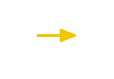
\begin{tikzpicture}[baseline]
    \node [anchor=base] (x) {};
    \draw [rawarrow] (x.mid west) -- ($(x.mid west) + (2em,0)$);
  \end{tikzpicture}
}

\newenvironment{slide}
{\begin{frame}[fragile,environment=slide]\vskip0pt plus 1filll}
{\vskip0pt plus 1filll\end{frame}}

% LaTeX

\setlength{\leftmargini}{1em}

% Common Information

\author{Talia Xu}
\course{COMPSCI 340}
\coursetitle{Operating Systems}
\date{2024 Semester 2}

% fontspec

\defaultfontfeatures{Ligatures=TeX}
% \setmainfont{Domine}
\setsansfont{Inter}[
  FontFace={ul}{n}{Font=*-Thin},
  FontFace={el}{n}{Font=*-ExtraLight},
  FontFace={l}{n}{Font=*-Light},
  FontFace={sb}{n}{Font=*-SemiBold},
  FontFace={eb}{n}{Font=*-ExtraBold},
  FontFace={xb}{n}{Font=*-Black},
]
\setmonofont[Contextuals=AlternateOff, Ligatures=TeXOff]{Iosevka}[
  FontFace={xb}{n}{Font=*-Heavy},
]

%% Font Weights

\DeclareRobustCommand{\ulseries}{\fontseries{ul}\selectfont}
\DeclareTextFontCommand{\textul}{\ulseries}
\DeclareRobustCommand{\elseries}{\fontseries{el}\selectfont}
\DeclareTextFontCommand{\textel}{\elseries}
\DeclareRobustCommand{\lseries}{\fontseries{l}\selectfont}
\DeclareTextFontCommand{\textl}{\lseries}
\DeclareRobustCommand{\sbseries}{\fontseries{sb}\selectfont}
\DeclareTextFontCommand{\textsb}{\sbseries}
\DeclareRobustCommand{\ebseries}{\fontseries{eb}\selectfont}
\DeclareTextFontCommand{\texteb}{\ebseries}
\DeclareRobustCommand{\xbseries}{\fontseries{xb}\selectfont}
\DeclareTextFontCommand{\textxb}{\xbseries}

% tikz

\usetikzlibrary{
  arrows,
  arrows.meta,
  automata,
  backgrounds,
  calc,
  decorations.pathreplacing,
  matrix,
  positioning,
  overlay-beamer-styles,
  shapes,
  shapes.multipart,
  tikzmark,
}

\tikzstyle{rawarrow} = [
  -{Latex[round]},
  line width=1pt,
  yellow,
  shorten >=3pt,
  shorten <=3pt,
  font=\small,
  text=black,
]

\tikzstyle{arrow} = [
  -{Latex[round]},
  line width=1pt,
  yellow,
  shorten >=3pt,
  shorten <=3pt,
  transform canvas={yshift=3pt},
  font=\small,
  text=black,
]

\newcommand{\tikzmarkcoord}[1]{([yshift=3pt]pic cs:#1)}

% minted

\setminted{style=eyolfson, fontsize=\small, escapeinside=||}
\setmintedinline{fontsize=\normalsize}

% hyperref

\hypersetup{colorlinks, urlcolor=blue}

% beamer
\setbeamersize{text margin left=16mm, text margin right=16mm}
\setbeamertemplate{itemize items}[circle]
\setbeamercolor{item}{fg=black}
\setbeamercolor{structure}{fg=darkblue}
\setbeamerfont{frametitle}{series=\bfseries, parent=structure}
\setbeamertemplate{navigation symbols}{}
\setbeamertemplate{headline}{}
\setbeamertemplate{footline}{
  \begin{tikzpicture}[
    remember picture,
    overlay,
    shift={(current page.south west)},
  ]
    \path [fill=gray] (144mm, 0) -- (160mm, 16mm) -- (160mm, 0);
    \node [inner sep=3.5mm, outer sep=0, text=black, anchor=base east,
           align=right, yshift=3.5mm]
          at (current page.south east) {\ttfamily \small \insertframenumber{}};
  \end{tikzpicture}
}
\setbeamertemplate{title page}{
  \begin{tikzpicture}[
    remember picture,
    overlay,
    shift={(current page.south west)},
    background rectangle/.style={fill=darkblue},
    show background rectangle,
  ]
    \node [anchor=center, align=center, text=white, text width=40mm, scale=3.2]
          at (\paperwidth / 2, \paperheight * 2 / 3)
          {\xbseries \inserttitle{}};
    \node [anchor=base west, align=left, inner sep=0, text=white, yshift=2.5mm]
          at (16mm, \paperheight / 3)
          {\insertdate{} \insertcourse{}: \insertcoursetitle{}};
    \node [anchor=base west, align=left, inner sep=0, text=white, yshift=-2.5mm]
          at (16mm, \paperheight / 3)
          {\insertauthor};
    \node [anchor=base east, align=right, inner sep=0, text=white, yshift=2.5mm]
          at (144mm, \paperheight / 3)
          {Lecture \insertlecturenumber{}};
    \node [anchor=base east, align=right, inner sep=0, text=white,
           yshift=-2.5mm]
          at (144mm, \paperheight / 3)
          {\ttfamily \insertversion{}};
    \node [align=center, anchor=south, inner sep=0, text=white, yshift=3.5mm]
          (license) at (\paperwidth / 2, 0)
          {\fontsize{7pt}{7pt}\selectfont This  work is licensed under a
           \href{http://creativecommons.org/licenses/by-sa/4.0/}
                {\color{lightblue} Creative Commons Attribution-ShareAlike 4.0
                 International License}};
  \end{tikzpicture}
}

% xcolor

%% Primary Colour

\definecolor{pantone655}{RGB}{0, 42, 92} % #002a5c
\colorlet{darkblue}{pantone655}

%% Secondary Colours

\definecolor{pantone633}{RGB}{0, 139, 176} % #008bb0
\colorlet{blue}{pantone633}

\definecolor{pantonewarmred}{RGB}{220, 70, 51} % #dc4633
\colorlet{red}{pantonewarmred}

\definecolor{pantone3285}{RGB}{0, 161, 137} % #00a189
\colorlet{cyan}{pantone3285}

\definecolor{pantone7722}{RGB}{13, 83, 77} % #0d534d
\colorlet{darkcyan}{pantone7722}

\definecolor{pantone376}{RGB}{141, 191, 46} % #8dbf2e
\colorlet{green}{pantone376}

\definecolor{pantone2613}{RGB}{109, 36, 122} % #6d247a
\colorlet{violet}{pantone2613}

\definecolor{pantone2985}{RGB}{111, 199, 234} % #6fc7ea
\colorlet{lightblue}{pantone2985}

\definecolor{pantone227}{RGB}{171, 19, 104} % #ab1368
\colorlet{magenta}{pantone227}

\definecolor{pantone7406}{RGB}{241, 197, 0} % #f1c500
\colorlet{yellow}{pantone7406}

%% Neutrals

\definecolor{pantonecoolgray2}{RGB}{208, 209, 201} % #d0d1c9
\colorlet{gray}{pantonecoolgray2}


\lecturenumber{1}
\title{Memory}
\version{1.0.0}

\begin{document}

\begin{frame}[plain, noframenumbering]
    \titlepage
\end{frame}

\begin{slide}

    \slidetitle{Not all virtual memory is mapped to physical memory}

    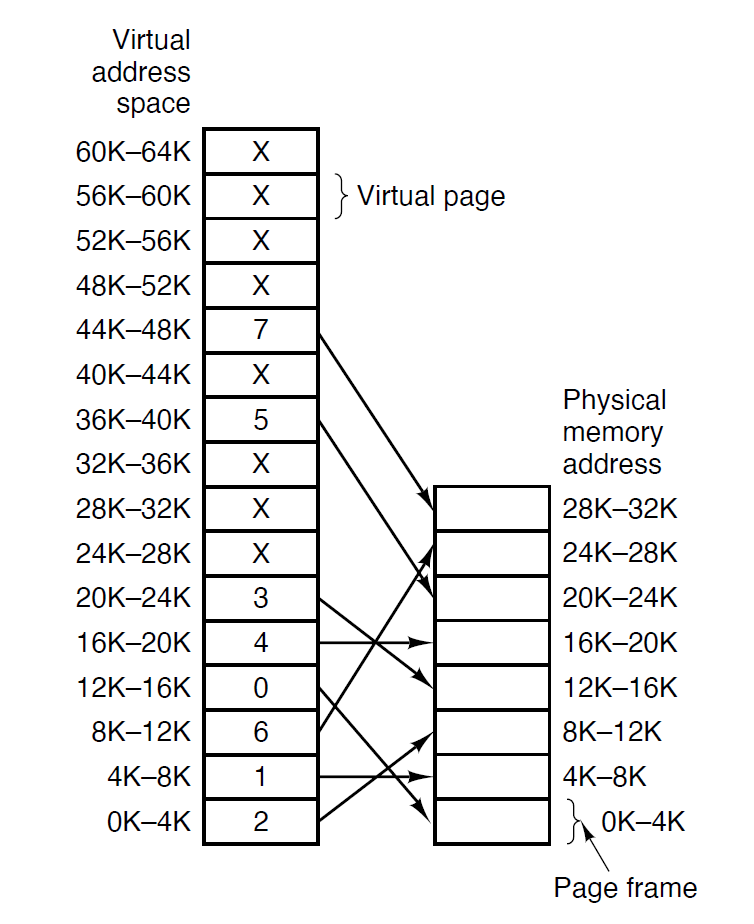
\includegraphics[width=50mm]{unmapped-mem.png}

\end{slide}

\begin{slide}
    
    \slidetitle{What Should We Do About the Page Table Size?}

    Most programs don't use all the virtual memory space, how can we take
    advantage?

\end{slide}
  
\begin{slide}
    
    \slidetitle{We Can Make Our Page Table Fit on a Page}

    \centering
    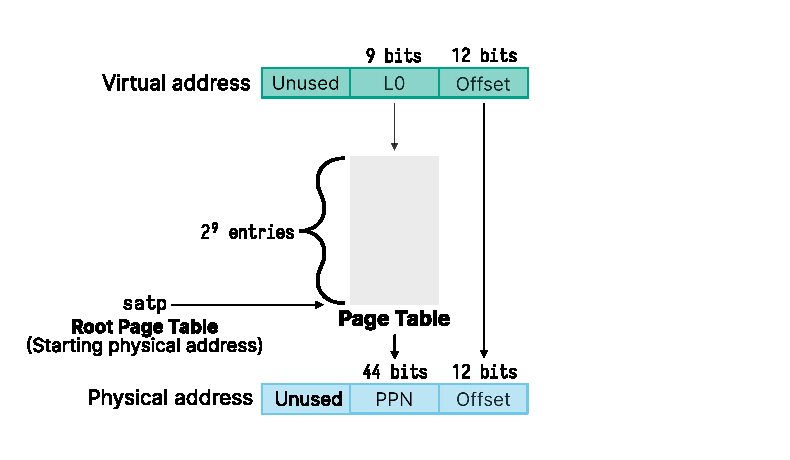
\includegraphics{single-level-page-table-small.eps}

\end{slide}

\begin{slide}

    \slidetitle{Multi-Level Page Tables Save Space for Sparse Allocations}

    \centering
    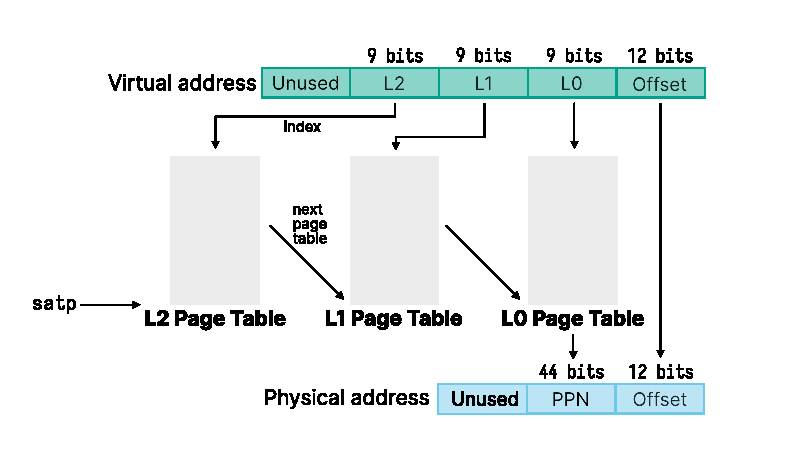
\includegraphics{multi-level-page-table.eps} 

\end{slide}

\begin{slide}

    \slidetitle{Page Allocation Uses A Free List}

    Given physical pages, the operating system maintains a free list (linked
    list)
    \medskip

    The unused pages themselves contain the \texttt{next} pointer in the free list

    \leftspace{}Physical memory gets initialized at boot
    \medskip

    To allocate a page, you remove it from the free list

    \leftspace{}To deallocate a page you add it back to the free list

\end{slide}

\begin{slide}

    \slidetitle{Insight: Use a Page for Each Smaller Page Table}

    There are 512 ($\mathsf{2^9}$) entries of 8 bytes($\mathsf{2^3}$) each,
    which is 4096 bytes
    \medskip

    The PTE for L(N) points to the page table for L(N-1)
    \medskip

    You follow these page tables until L0 and that contains the \texttt{PPN}

\end{slide}

\begin{slide}
    
    \slidetitle{The Smaller Page Tables are Just Like Arrays}

    Instead of:

    \leftspace{}\mintinline{c}{int page_table[512] // What's the size of this?}

    or

    \leftspace{}%
    \mintinline{c}{x = page_table[2]; // What's the offset of index 2?}
    \medskip

    You have:

    \leftspace{}\mintinline{c}{PTE page_table[512]}

    where:

    \leftspace{}\mintinline{c}{sizeof(page_table) == PAGE_SIZE}

    and

    \leftspace{}%
    \mintinline{c}{sizeof(page_table) = number of entries * sizeof(PTE)}

\end{slide}

\begin{slide}

    \slidetitle{Consider Just One Additional Level}

    Assume our process uses just one virtual address at \texttt{0x3FFFF008}

    \leftspace{}or \texttt{0b11\_1111\_1111\_1111\_1111\_0000\_0000\_1000}

    \leftspace{}or \texttt{0b111111111\_111111111\_000000001000}
    \medskip

    We'll just consider a 30-bit virtual address with a page size of 4096 bytes

    \leftspace{}We would need a 2 MiB page table if we only had one
    ($\mathsf{2^{18} \times 2^{3}}$)
    \medskip

    Instead, we have a 4 KiB L1 page table ($\mathsf{2^9 \times 2^{3}}$) and a 4
    KiB L0 page table

    \leftspace{}Total of 8 KiB instead of 2 MiB
    \medskip

    Note: worst case if we used all virtual addresses we would consume 2 MiB + 4
    KiB

\end{slide}

\begin{slide}

    \slidetitle{Translating \texttt{3FFFF008} with 2 Page Tables}

    Consider the L1 table with the entry:

	\begin{center}
		{\ttfamily
		\begin{tabular}{rl}
		  Index & PPN \\
		  511   & 0x8 \\
		\end{tabular}}
		\end{center}
		\medskip

		Consider the L0 table located at \texttt{0x8000} with the entry:
		\begin{center}
		{\ttfamily
		\begin{tabular}{rl}
		  Index & PPN \\
		  511   & 0xCAFE \\
		\end{tabular}}
    \end{center}
    
    The final translated physical address would be: \texttt{0xCAFE008}

\end{slide}
  
\end{document}
